\documentclass[10pt, conference, compsocconf]{IEEEtran}
\usepackage{amsmath,color,graphicx}

% *** GRAPHICS RELATED PACKAGES ***
%
\ifCLASSINFOpdf
  % \usepackage[pdftex]{graphicx}
  % declare the path(s) where your graphic files are
  % \graphicspath{{../pdf/}{../jpeg/}}
  % and their extensions so you won't have to specify these with
  % every instance of \includegraphics
  % \DeclareGraphicsExtensions{.pdf,.jpeg,.png}
\else
  % or other class option (dvipsone, dvipdf, if not using dvips). graphicx
  % will default to the driver specified in the system graphics.cfg if no
  % driver is specified.
  % \usepackage[dvips]{graphicx}
  % declare the path(s) where your graphic files are
  % \graphicspath{{../eps/}}
  % and their extensions so you won't have to specify these with
  % every instance of \includegraphics
  % \DeclareGraphicsExtensions{.eps}
\fi
% graphicx was written by David Carlisle and Sebastian Rahtz. It is
% required if you want graphics, photos, etc. graphicx.sty is already
% installed on most LaTeX systems. The latest version and documentation can
% be obtained at: 
% http://www.ctan.org/tex-archive/macros/latex/required/graphics/
% Another good source of documentation is "Using Imported Graphics in
% LaTeX2e" by Keith Reckdahl which can be found as epslatex.ps or
% epslatex.pdf at: http://www.ctan.org/tex-archive/info/
%
% latex, and pdflatex in dvi mode, support graphics in encapsulated
% postscript (.eps) format. pdflatex in pdf mode supports graphics
% in .pdf, .jpeg, .png and .mps (metapost) formats. Users should ensure
% that all non-photo figures use a vector format (.eps, .pdf, .mps) and
% not a bitmapped formats (.jpeg, .png). IEEE frowns on bitmapped formats
% which can result in "jaggedy"/blurry rendering of lines and letters as
% well as large increases in file sizes.
%
% You can find documentation about the pdfTeX application at:
% http://www.tug.org/applications/pdftex





% *** MATH PACKAGES ***
%
%\usepackage[cmex10]{amsmath}
% A popular package from the American Mathematical Society that provides
% many useful and powerful commands for dealing with mathematics. If using
% it, be sure to load this package with the cmex10 option to ensure that
% only type 1 fonts will utilized at all point sizes. Without this option,
% it is possible that some math symbols, particularly those within
% footnotes, will be rendered in bitmap form which will result in a
% document that can not be IEEE Xplore compliant!
%
% Also, note that the amsmath package sets \interdisplaylinepenalty to 10000
% thus preventing page breaks from occurring within multiline equations. Use:
%\interdisplaylinepenalty=2500
% after loading amsmath to restore such page breaks as IEEEtran.cls normally
% does. amsmath.sty is already installed on most LaTeX systems. The latest
% version and documentation can be obtained at:
% http://www.ctan.org/tex-archive/macros/latex/required/amslatex/math/





% *** SPECIALIZED LIST PACKAGES ***
%
%\usepackage{algorithmic}
% algorithmic.sty was written by Peter Williams and Rogerio Brito.
% This package provides an algorithmic environment fo describing algorithms.
% You can use the algorithmic environment in-text or within a figure
% environment to provide for a floating algorithm. Do NOT use the algorithm
% floating environment provided by algorithm.sty (by the same authors) or
% algorithm2e.sty (by Christophe Fiorio) as IEEE does not use dedicated
% algorithm float types and packages that provide these will not provide
% correct IEEE style captions. The latest version and documentation of
% algorithmic.sty can be obtained at:
% http://www.ctan.org/tex-archive/macros/latex/contrib/algorithms/
% There is also a support site at:
% http://algorithms.berlios.de/index.html
% Also of interest may be the (relatively newer and more customizable)
% algorithmicx.sty package by Szasz Janos:
% http://www.ctan.org/tex-archive/macros/latex/contrib/algorithmicx/




% *** ALIGNMENT PACKAGES ***
%
%\usepackage{array}
% Frank Mittelbach's and David Carlisle's array.sty patches and improves
% the standard LaTeX2e array and tabular environments to provide better
% appearance and additional user controls. As the default LaTeX2e table
% generation code is lacking to the point of almost being broken with
% respect to the quality of the end results, all users are strongly
% advised to use an enhanced (at the very least that provided by array.sty)
% set of table tools. array.sty is already installed on most systems. The
% latest version and documentation can be obtained at:
% http://www.ctan.org/tex-archive/macros/latex/required/tools/


%\usepackage{mdwmath}
%\usepackage{mdwtab}
% Also highly recommended is Mark Wooding's extremely powerful MDW tools,
% especially mdwmath.sty and mdwtab.sty which are used to format equations
% and tables, respectively. The MDWtools set is already installed on most
% LaTeX systems. The lastest version and documentation is available at:
% http://www.ctan.org/tex-archive/macros/latex/contrib/mdwtools/


% IEEEtran contains the IEEEeqnarray family of commands that can be used to
% generate multiline equations as well as matrices, tables, etc., of high
% quality.


%\usepackage{eqparbox}
% Also of notable interest is Scott Pakin's eqparbox package for creating
% (automatically sized) equal width boxes - aka "natural width parboxes".
% Available at:
% http://www.ctan.org/tex-archive/macros/latex/contrib/eqparbox/





% *** SUBFIGURE PACKAGES ***
%\usepackage[tight,footnotesize]{subfigure}
% subfigure.sty was written by Steven Douglas Cochran. This package makes it
% easy to put subfigures in your figures. e.g., "Figure 1a and 1b". For IEEE
% work, it is a good idea to load it with the tight package option to reduce
% the amount of white space around the subfigures. subfigure.sty is already
% installed on most LaTeX systems. The latest version and documentation can
% be obtained at:
% http://www.ctan.org/tex-archive/obsolete/macros/latex/contrib/subfigure/
% subfigure.sty has been superceeded by subfig.sty.



%\usepackage[caption=false]{caption}
%\usepackage[font=footnotesize]{subfig}
% subfig.sty, also written by Steven Douglas Cochran, is the modern
% replacement for subfigure.sty. However, subfig.sty requires and
% automatically loads Axel Sommerfeldt's caption.sty which will override
% IEEEtran.cls handling of captions and this will result in nonIEEE style
% figure/table captions. To prevent this problem, be sure and preload
% caption.sty with its "caption=false" package option. This is will preserve
% IEEEtran.cls handing of captions. Version 1.3 (2005/06/28) and later 
% (recommended due to many improvements over 1.2) of subfig.sty supports
% the caption=false option directly:
%\usepackage[caption=false,font=footnotesize]{subfig}
%
% The latest version and documentation can be obtained at:
% http://www.ctan.org/tex-archive/macros/latex/contrib/subfig/
% The latest version and documentation of caption.sty can be obtained at:
% http://www.ctan.org/tex-archive/macros/latex/contrib/caption/




% *** FLOAT PACKAGES ***
%
%\usepackage{fixltx2e}
% fixltx2e, the successor to the earlier fix2col.sty, was written by
% Frank Mittelbach and David Carlisle. This package corrects a few problems
% in the LaTeX2e kernel, the most notable of which is that in current
% LaTeX2e releases, the ordering of single and double column floats is not
% guaranteed to be preserved. Thus, an unpatched LaTeX2e can allow a
% single column figure to be placed prior to an earlier double column
% figure. The latest version and documentation can be found at:
% http://www.ctan.org/tex-archive/macros/latex/base/



%\usepackage{stfloats}
% stfloats.sty was written by Sigitas Tolusis. This package gives LaTeX2e
% the ability to do double column floats at the bottom of the page as well
% as the top. (e.g., "\begin{figure*}[!b]" is not normally possible in
% LaTeX2e). It also provides a command:
%\fnbelowfloat
% to enable the placement of footnotes below bottom floats (the standard
% LaTeX2e kernel puts them above bottom floats). This is an invasive package
% which rewrites many portions of the LaTeX2e float routines. It may not work
% with other packages that modify the LaTeX2e float routines. The latest
% version and documentation can be obtained at:
% http://www.ctan.org/tex-archive/macros/latex/contrib/sttools/
% Documentation is contained in the stfloats.sty comments as well as in the
% presfull.pdf file. Do not use the stfloats baselinefloat ability as IEEE
% does not allow \baselineskip to stretch. Authors submitting work to the
% IEEE should note that IEEE rarely uses double column equations and
% that authors should try to avoid such use. Do not be tempted to use the
% cuted.sty or midfloat.sty packages (also by Sigitas Tolusis) as IEEE does
% not format its papers in such ways.





% *** PDF, URL AND HYPERLINK PACKAGES ***
%
%\usepackage{url}
% url.sty was written by Donald Arseneau. It provides better support for
% handling and breaking URLs. url.sty is already installed on most LaTeX
% systems. The latest version can be obtained at:
% http://www.ctan.org/tex-archive/macros/latex/contrib/misc/
% Read the url.sty source comments for usage information. Basically,
% \url{my_url_here}.





% *** Do not adjust lengths that control margins, column widths, etc. ***
% *** Do not use packages that alter fonts (such as pslatex).         ***
% There should be no need to do such things with IEEEtran.cls V1.6 and later.
% (Unless specifically asked to do so by the journal or conference you plan
% to submit to, of course. )


% correct bad hyphenation here
\hyphenation{op-tical net-works semi-conduc-tor}


\begin{document}
%
% paper title
% can use linebreaks \\ within to get better formatting as desired
\title{
    Towards Optimal Snapshot Materialization \\
    To Support Large Query Workload For 
    Append-only Temporal Databases
}


\author{
    \IEEEauthorblockN{ Amin Beirami }
    \IEEEauthorblockA{
        Faculty of Science \\
        UOIT \\
        Oshawa, Canada \\
        beirami.m.a@gmail.com
    }
    \and
    \IEEEauthorblockN{Ken Pu}
    \IEEEauthorblockA{
        Faculty of Science \\
        UOIT \\
        Oshawa, Canada \\
        ken.pu@uoit.ca
    }
    \and
    \IEEEauthorblockN{Ying Zhu}
    \IEEEauthorblockA{
        Faculty of Business & IT \\
        UOIT \\
        Oshawa, Canada \\
        ying.zhu@uoit.ca
    }
}

% make the title area
\maketitle


\begin{abstract}
    We present several results on optimal snapshot materialization
    for append-only temporal databases in order to support very large
    scale query workload.  Our data model is temporal relational data
    stored in an append-only database.  In the presence of multiple
    and concurrent queries over the timeline of the temporal database,
    recomputing snapshots of the entire database at the timestamp of
    interesting of each query is computationally expensive and inefficient.

    In this paper, we present a practical solution to support large query load
    by materializing $m$ snapshots at optimal timestamps.  We show that optimal
    snapshot timestamps can be computed efficiently in {\em linear time}.
    We further show that with varying query load, we can dynamically adjust
    snapshots to adjust to the changin query load.
\end{abstract}

\begin{IEEEkeywords}
temporal databases; materialized views; query workload; optimization
\end{IEEEkeywords}


% For peer review papers, you can put extra information on the cover
% page as needed:
% \ifCLASSOPTIONpeerreview
% \begin{center} \bfseries EDICS Category: 3-BBND \end{center}
% \fi
%
% For peerreview papers, this IEEEtran command inserts a page break and
% creates the second title. It will be ignored for other modes.
\IEEEpeerreviewmaketitle


\newtheorem{example}{Example}
\newtheorem{definition}{Definition}
\newtheorem{prop}{Proposition}

\section{Introduction}

Recently, as part of the Big Data movement,
information systems have been designed to archive every bit of 
data over time. In contrast to traditional data warehouse databases, modern
databases are aimed to store {\em every} update, insert and deletion as a
transaction.

\begin{example}
    Consider the following table {\tt Products} which stores the product
    information.

    \vspace{1em}

    \begin{center}
        \small
        \begin{tabular}{|c|c|c|c|} \hline
            id & part-name & Manufacture & Price \\ \hline
            0010 & Game Console &  Nintendo & \$399 \\ \hline
            0011 & Keyboard &  Microsoft & \$89 \\ \hline
            $\vdots$ & \vdots & \vdots & \vdots \\ \hline
        \end{tabular}
    \end{center}

    \vspace{1em}

    Suppose that there will be frequent updates to the products such as
    addition of new products, renaming of existing products, and price
    adjustments. The {\tt product} table can only store the eventual state of
    the database {\em after} each updates, but not the updates themselves.  The
    update transactions are quite valuable themselves.

    We would like to augment the database schema to make {\tt product} into a
    {\em temporal} table which we will call $\mathtt{product}^T$. The temporal
    table is to store {\em all} modifications to the {\tt product} table.
    Hence, it has the following schema:

    \vspace{1em}
    \begin{center}
        \small
        \begin{tabular}{|c|c|c|c|c|c|} \hline
            :updates: & :deleted: & id & part-name & Manufacture & Price \\ \hline
            00000001 & false & 0010 & Game Console & Nintendo & \$359 \\ \hline
            00000002 & false & 0020 & Monitor & Samsung & \$159 \\ \hline
            00000003 & false & 0010 & Game Console & Nintendo & \$399 \\ \hline
            00000004 & true & 0011 & - & - & - \\ \hline
            $\vdots$ & $\vdots$ & $\vdots$ & $\vdots$ & $\vdots$ &  $\vdots$ \\ \hline
        \end{tabular}
    \end{center}
    \vspace{1em}

    It shows four specific updates done to the {\tt product} table:

    \begin{itemize}
        \item The {\em game console} is discounted to a new price \$359.
        \item A new product {\em Monitor} is added to the table.
        \item The {\em game console} is no longer on sale, so its price is back
            to \$399.
        \item The keyboard (product ID 0011) is discontinued, so it's deleted
            from the table.
    \end{itemize}

\end{example}


\newcommand{\attr}{\mathrm{attr}}

\section{Problem Definition}

\begin{definition}[Temporal database]
    Let $r_1, r_2, \dots r_n$ be the tables
    in a database $D$.  Denote the attributes
    of each table as $\attr(r_i)$.

    A temporal table, denoted $r_i^T$, is
    a table with the attributes:

    $$\attr(r_i^T) = \{\mathrm{updates}, \mathrm{deleted}\} \cup \attr(r_i)$$

    By a temporal database, we mean the database obtained by augmenting
    $D$ by the temporal tables:

    $$ D^T = D \cup \{r_i^T: r_i\in D\} $$
\end{definition}

There is a lot of value in maintaining $D^T$ because it stores the entire update
history of $D$.  Traditionally, this may be seen as an overly burdening task,
but that is no longer the case with increasingly affordable cloud storage
solutions.  Furthermore, the update history provides many valuable insights into
the dynamics of data. We are motivated to support queries for the database at a
specific time.

\begin{definition}[Snapshots and queries]
    Given a temporal table $r^T$, and a timestamp $t$, we denote
    $r(t)$ to be the table instance obtained by applying the updates
    in $r^T$ where $r^T[\mathrm{updates}] \leq t$.

    A snapshot is a materialized version of $D(t) = \{r_1(t), r_2(t), \dots,
    r_n(t)\}$.  A snapshot query is an arbitrary relational query on $D(t)$.
\end{definition}

We can construct the snapshots using simple windowing functions (as in supported
by PostgreSQL \cite{momjian2001postgresql}).


\vspace{1em}

{\small
\begin{tabular}{|l|} \hline
    $\mathrm{snapshot}(r, t)$ = \\
    \verb|| \textsc{With} $T$ \textsc{as} ( \\
    \verb| | \textsc{select} id, $\{\mathrm{last\_value}(x) \mathrm{\ as\ } x:
    x\in\attr(r)\}$ \textsc{over} $W$ \\
    \verb| | \textsc{from} $r^T$ \\
    \verb| | \textsc{where} updates $\leq t$ \\
    \verb| | \textsc{window} $W$ \textsc{as} 
             \textsc{partition by} id \textsc{order by} updates\\
    \verb|| ) \\
    \verb|| \textsc{select} id, $\{x: x\in\attr(r)\}$ \textsc{from} $T$ \\
    \verb|| \textsc{where not} $T.$deleted \\ \hline
\end{tabular}
}

\vspace{1em}

The query $\mathrm{snapshot}(r, t)$ computes the snapshot of $r$ at timestamp
$t$ by applying the latest update of each tuple up to timestamp $t$, while
removing tuples that have been deleted.

\begin{prop}
    \label{prop:linear-time}
    Assume that the tables are updated at a constant rate over time,
    then the complexity of $\mathrm{snapshot}(r, t)$ is 
    $$\mathcal{O}(|\{x: x\in r^T\mathrm{\ and\ } x.\mathrm{updates} \leq t\}|)
    \simeq \mathcal{O}(t)$$
\end{prop}

\subsection{Query answering using snapshots}

Using precomputed materialized view has been shown to be highly effective \cite{sohrabi2016materialized,du2017deepsea}.
Thus, in order to answer a query $Q(t)$ on $D(t)$, we propose to first precompute
snapshots $\mathrm{snapshot}(r, t)$ and then evaluate $Q$.  If some snapshots
are precomputed and materialized, then we can save on the computational cost in
answering the query $Q(t)$.

\begin{prop}
    Let $r$ be a temporal relation, with $s$ and $t$ being timestamps.
    Suppose we have materialized $\mathrm{snapshot}(r, s)$.  Then
    $\mathrm{snapshot}(r, t)$ can be computed with complexity:

    $$\mathcal{O}(|\{x: x\in r^T\mathrm{\ and\ } x.\mathrm{updates} \in [s,
    t]\}|) \simeq \mathcal{O}(|s-t|)$$
\end{prop}

\subsection{Optimal materialization of snapshots}

We define the central problems of this paper, namely computing the timestamps at
which we can materialize the snapshots to best answer a given query workload.
Let $T_Q = \{q_1, q_2, \dots, q_n\}$ be the timestamps of $n$ queries, each 
querying the database at $D(q_i)$.  We define the cost functions as the total
query answering cost given some precomputed and materialized snapshots.

\begin{definition}[Query answering cost]
    Suppose that a single snapshot at time $s$ is materialized, then
    $$\mathrm{cost}(T_Q | s) = \sum_{q\in T_Q} |q - s|$$

    If we have multiple snapshots at times $S=\{s_1, s_2, \dots, s_m\}$
    materialized, then

    $$\mathrm{cost}(T_Q|S) = \sum_{q\in T_Q} \min\{|q-s| : s\in S\}$$
\end{definition}

\begin{definition}[Optimal snapshot placement]
    The {\em single snapshot placement} problem is
    to compute the timestamp $s^*$ such that $\mathrm{cost}(T_Q | s)$ is
    minimized.

    The {\em $m$-snapshots placement} problem is
    to compute a set of timestamps $S^* = \{s_1, s_2, \dots s_m\}$
    such that $\mathrm{cost}(T_Q | S)$ is minimized.
\end{definition}

In the remainder of the paper, we present the algorithms and experimental
evaluation to demonstrate that the optimal snapshot placement problems can be
efficiently solved, and that their solutions yield a practical solution to
support queries of temporal databases.

\begin{figure}[tb]
    \label{fig:query-time-no-snap}
    \centering
    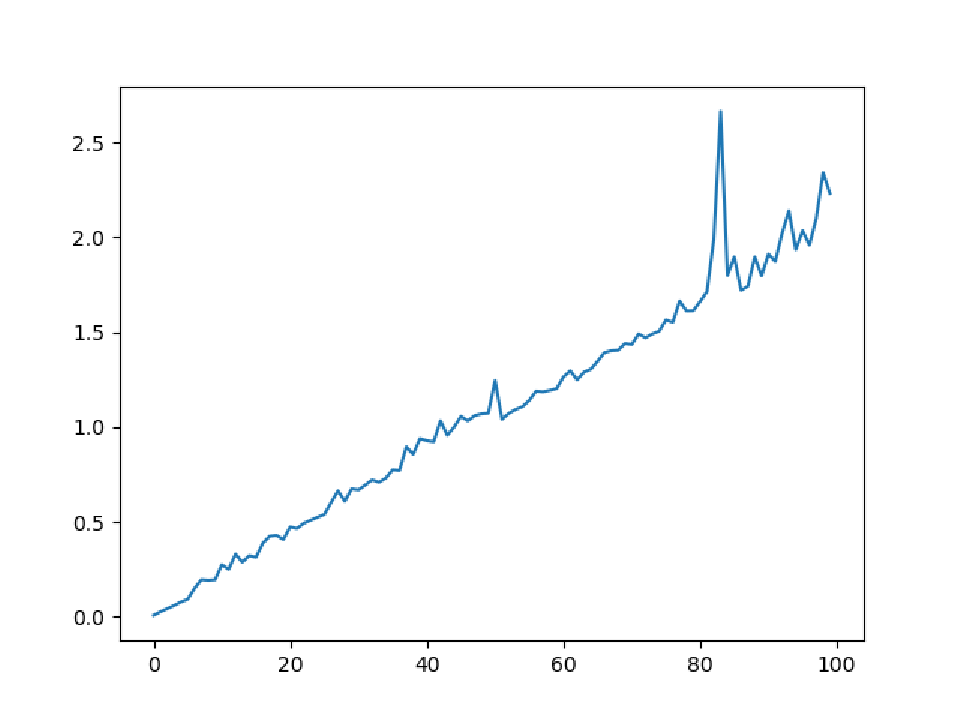
\includegraphics[width=2.8in]{figs/runtime.pdf}
    \caption{Query answering for 100 queries without snapshots.}
\end{figure}




\section{Algorithm}

We first solve the simpler single snapshot placement problem.

\begin{prop}
    \label{thm:single}
    The single snapshot placement problem can be solved in $\mathcal{O}(|T_Q|)$,
    with the optimal snapshot placement at
    $ s^*(T_Q) = \mathrm{median}(T_Q) $,
    which can be computed in $\mathcal{O}(|T_Q|)$.
\end{prop}

%\textcolor{red}{Proof [Outline]}

So by Proposition~\ref{thm:single}, it's straightforward to compute the optimal
placement of a single snapshot with respect to a given query workload.  However,
in practice, we want to allocate a number, $m$, of snapshots to be placed, where
$m$ is a determined by the available resource.
In this section, we extend Proposition~\ref{thm:single} to handle arbitrary number
of snapshots.

First we will present an recursive algorithm that solves the optimal
$m$-snapshot placement problem.

Without loss of generality, let's assume that  the query timestamps are sorted
in $Q = \{q_1, q_2, \dots, q_n\}$.  Here $Q$ is the sorted list of query
timestamps.  We denote $Q[i,j] = \{q_i, q_{i+1}, \dots, q_{j-1}, q_j\}$.

The objective is to compute $S = \{s_1, s_2, \dots, s_m\}$ such
that the query answering time given by $\mathrm{cost}(Q|S)$ is minimized.

\begin{prop}[Segmentation of queries]
    \label{thm:seg}
    Given any snapshot timestamps in a sorted order $S = \{s_1, s_2, \dots,
    s_m\}$ such that $s_i\leq s_{i+1}$, the snapshots partition the queries $Q$
    into $m$ non-overlapping segments $Q[1, i_1], Q[i_1+1, i_2], \dots
    Q[i_{m-1}, i_m]$ such that queries in $Q[i_j, i_{j+1}]$ uses $s_j$
    in the optimal query answer strategy.
\end{prop}

Proposition~\ref{thm:seg} allows us to construct a dynamic programming algorithm
that computes the {\em exact} optimal snapshot placements.

\subsection{Recursive formulation}
\label{sec:recursive}

Let $\mathrm{opt}(Q, m)$ be the optimal $m$-snapshot placements for the query
workload $Q$.

\begin{prop}[Optimality of sub-problems]
    \label{thm:subopt}
    Let $S^* = \mathrm{opt}(Q, m)$.  Let $\mathcal{Q}$ be the partition
    of segments created by $S^*$.  Then, the prefix of $S^*$ is also an optimal
    $m-1$ snapshot placement of the prefix of $\mathcal{Q}$.  Formally,

    $$\mathrm{prefix}(S^*) = \mathrm{opt}(\cup\mathrm{prefix}(\mathcal{Q}), m-1)$$
\end{prop}

We can formulate a recursive definition of $\mathrm{opt}(Q, m)$ using
Proposition~\ref{thm:subopt}.  The intuition is that we try out all possible
{\em last} segment of $Q$, and pick the one with the lowest cost.

The recursive definition of $\mathrm{opt}(Q, m)$ is given as:

\begin{itemize}
    \item Base case $ \mathrm{opt}(Q, 1) = \{\mathrm{median}(Q)\}$.
    \item Induction on $m$:
    $$i^* = \mathrm{argmin}\{\mathrm{cost}(\mathrm{opt}(Q[1,i], m-1)): i\in[1,
    n]\}$$
    $$
    \mathrm{opt}(Q, m) = \mathrm{opt}(Q[1, i^*]) \cup \{\mathrm{median}(Q[i^*+1, n])
    $$
\end{itemize}

\begin{prop}
    The recursive formulation of $\mathrm{opt}(Q, m)$ requires
    $\mathcal{O}(2^{m})$.
\end{prop}

Fortunately, we are able implement $\mathrm{opt}(Q, m)$ in polynomial time as a
dynamic programming problem.

\subsection{Dynamic programming formulation}
\label{sec:dynamic}

We can build a table $\mathbf{OPT}$ as a two dimensional array
indexed by $(i, k)$ where $i\in [1, n]$ and $k\in [1, m]$.  Each entry
in the table $\mathbf{OPT}[i,k] = \mathrm{opt}(Q[1,i], k)$.
We can compute $\mathbf{OPT}[i,k]$ in a bottom up fashion \cite{kossmann2000iterative}.

\vspace{1em}
{\small
\begin{tabular}{|l|} \hline
    computeOPT($Q$, $m$) = \\
    \verb|| $n = |Q|$ \\
    \verb|| $\mathbf{OPT}[i, 0] = \infty$ \\
    \verb|| for $k = 1 \to m$ \\
    \verb| | for $i = 1 \to n$ \\
    \verb|  | $j^* = \underset{j\in[1,i]}{\mathrm{argmin}}
                (\mathrm{cost}(\mathbf{OPT}[j,k-1]) + \mathrm{cost}(Q[j+1, n]))$ \\
    \verb|  | $\mathbf{OPT}[i,k] = \mathbf{OPT}[j^*, k-1] \cup \{\mathrm{median}(Q[j+1], n)\}$ \\
    \verb| | end for \\
    \verb|| end for \\ \hline
\end{tabular}
}
\vspace{1em}

\begin{prop}
    The complexity of computing all the entries of $\mathbf{OPT}$ is
    $\mathcal{O}(mn^2)$.
\end{prop}


\section{Experimental Evaluation}

\begin{figure}[tb]
    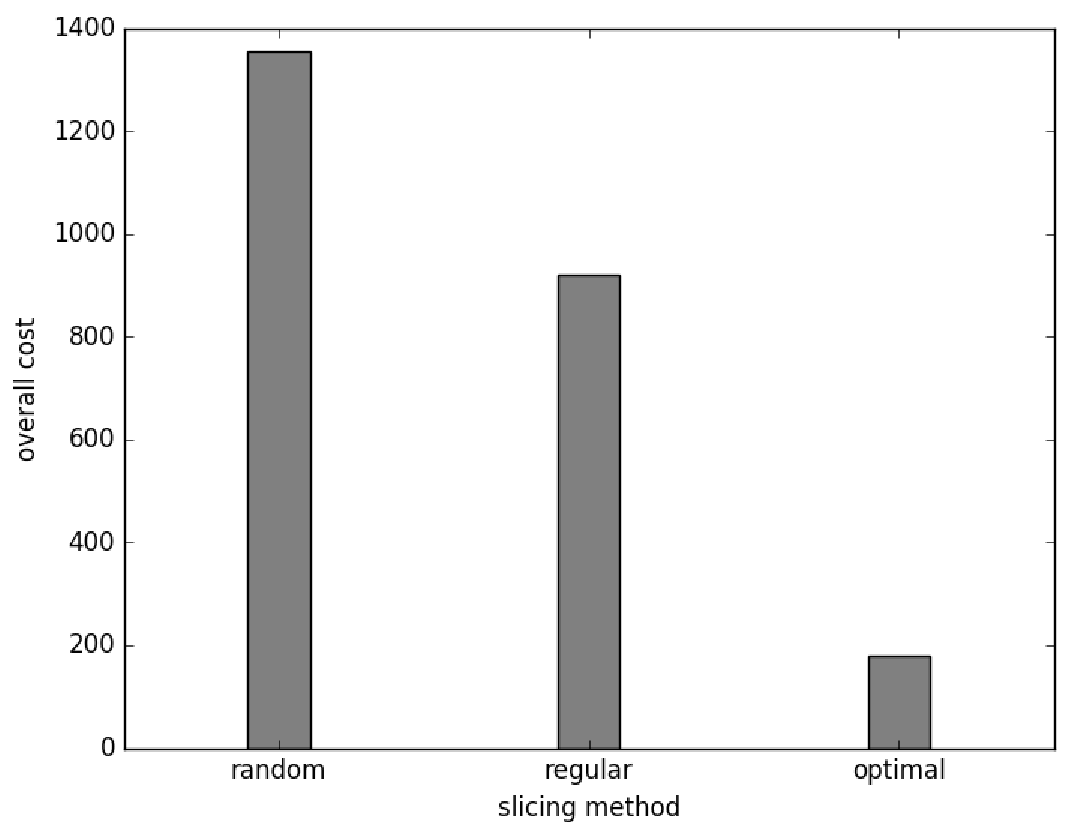
\includegraphics[width=3in]{figs/cuts_cost.pdf}
    \caption{Relative query answering cost}
\end{figure}

\begin{figure}[tb]
    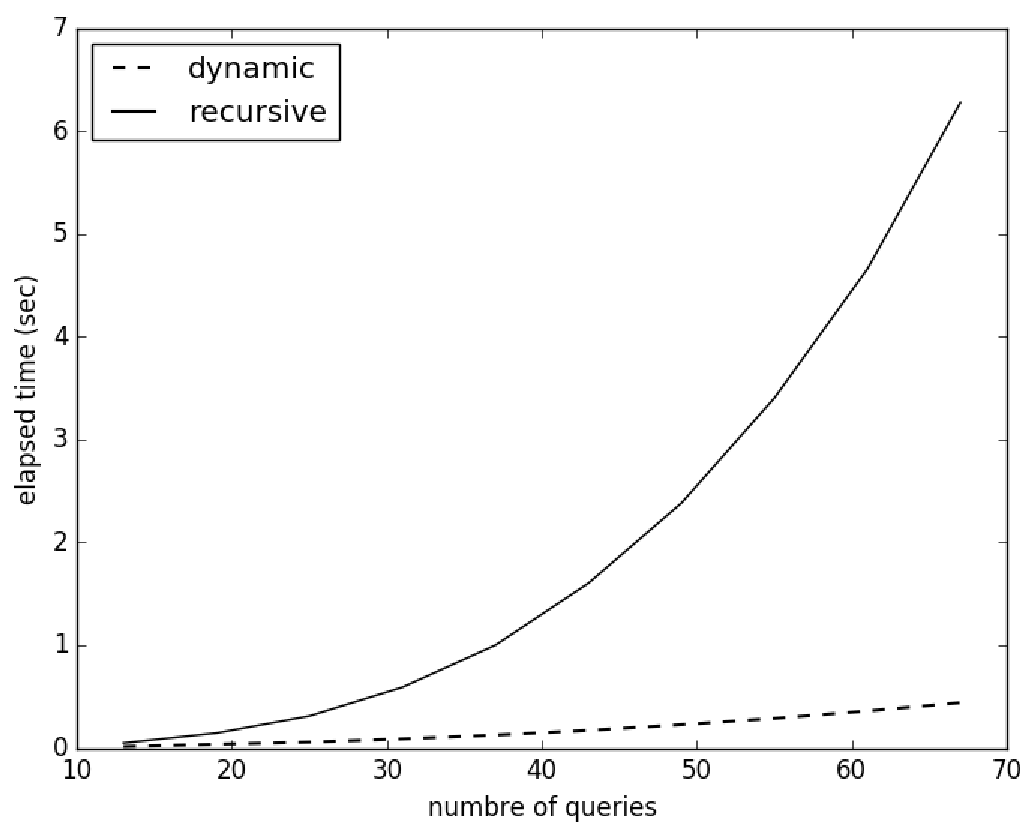
\includegraphics[width=3in]{figs/multiquery_runtime.pdf}
    \caption{Optimization time with respect to the number of queries}
\end{figure}

\begin{figure}[tb]
    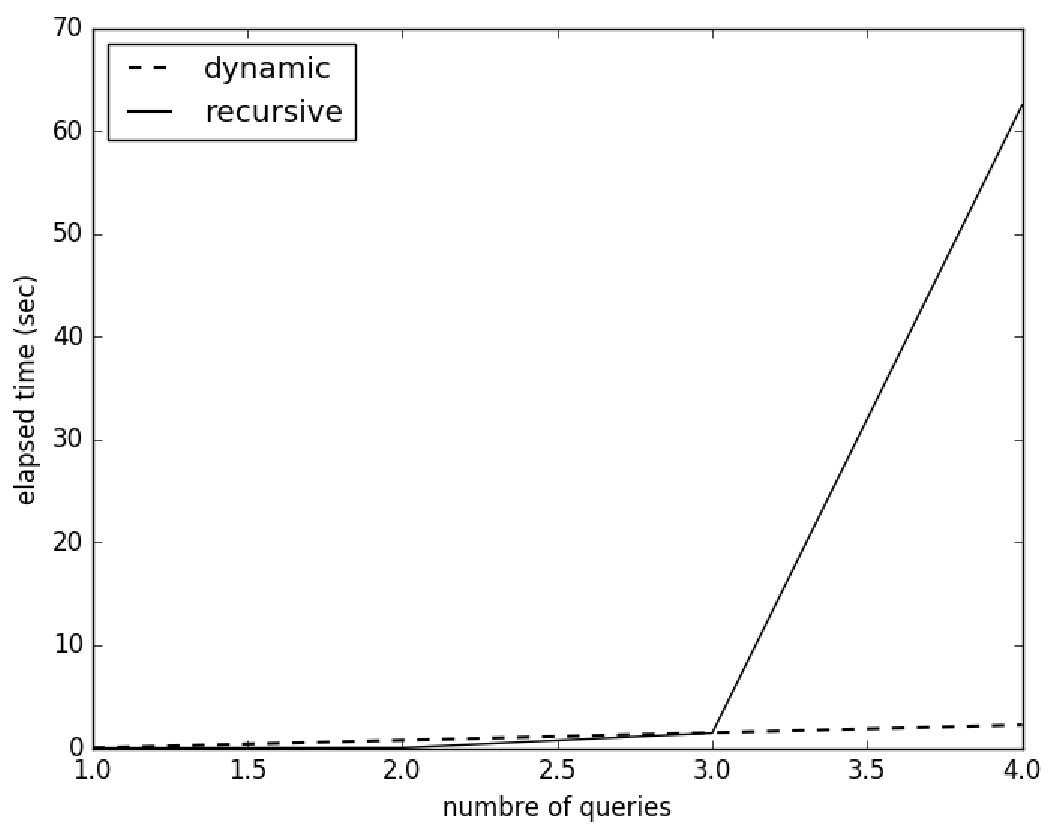
\includegraphics[width=3in]{figs/multisnap_runtime.pdf}
    \caption{Optimization time with respect to the number of snapshots}
\end{figure}

\begin{figure}[tb]
    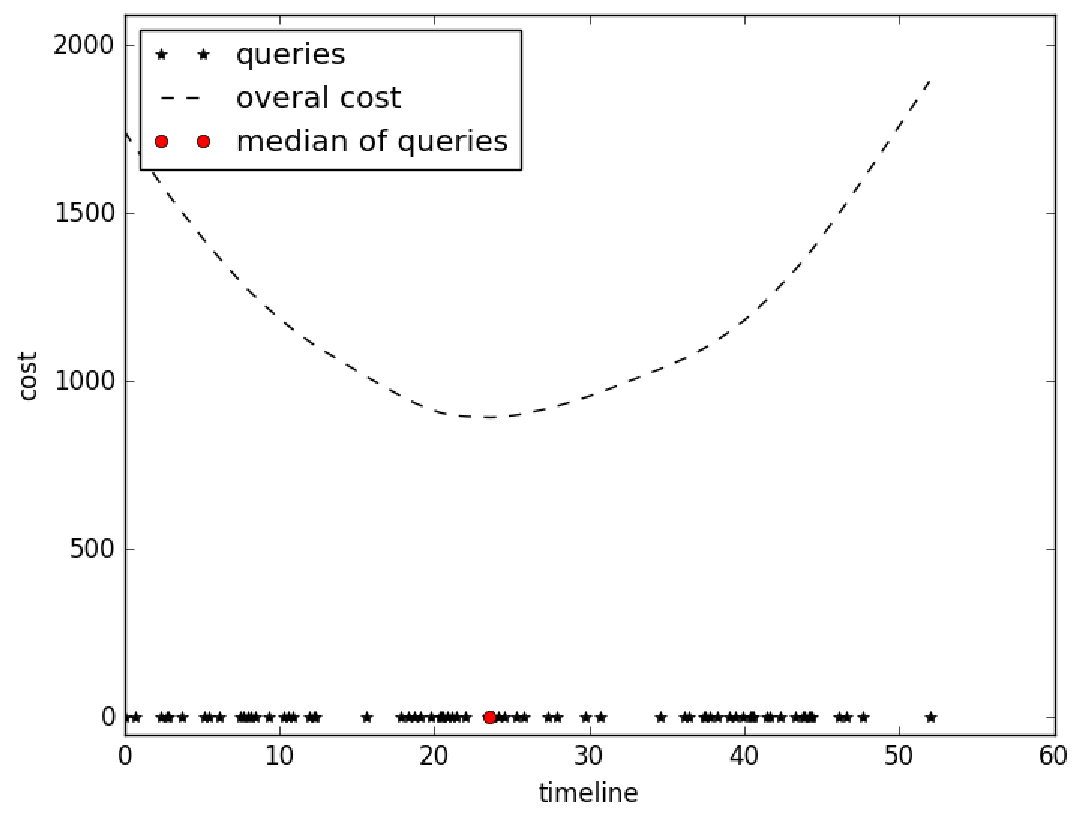
\includegraphics[width=3in]{figs/single.pdf}
    \caption{Cost of query answering using a single snapshot over different
    snaptshot timestamps}
\end{figure}

\begin{figure}[tb]
    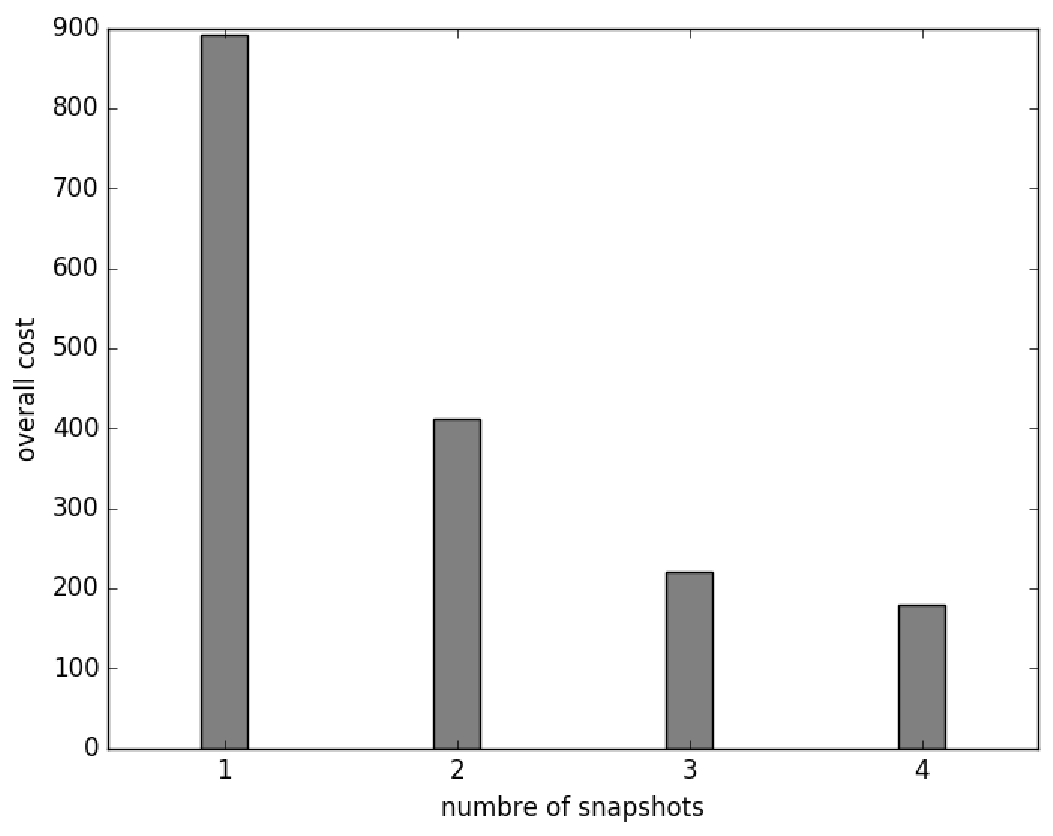
\includegraphics[width=3in]{figs/snap_cost.pdf}
    \caption{Query answering cost with increasing number of snapshots}
\end{figure}

\section{Conclusion and Future Work}

In this paper, we have presented some results obtained toward optimally
supporting temporal relational queries of databases that store the timelines of
its relational tables.  In order to avoid recomputation of the database states
while making use of the storage space efficiently, our solution is to
materialize $m$ snapshots at well-chosen timestamps.

We have constructed a model to describe the query answering cost, and this cost
model allows us to formulate the $m$-snapshot placement problem as an
optimization problem.  We showed that dynamic programming can be used to solve
the problem {\em exactly}.  Our experimental evaluation demonstrates that our
cost model agrees with relational database systems, and that our snapshot
placements improve query processing significantly.

This is on-going research. As future work, we will be investigating
approximation methods to further speed up the snapshot placement calculuation.
We also wish to investigate maintaining snapshot placement dynamically to cope
with a dynamic query workload.


\bibliographystyle{IEEEtran}
\bibliography{references}

% that's all folks
\end{document}
